\section{From automaton to regular expression: the BMC method}

Suppose for simplicity the initial state $i$ is unique, and no arc enters in it; similarly the final state $t$ is unique and without outgoing arcs. Otherwise, just add
a new initial state $i$ connected by spontaneous moves to the ex-initial states; similarly introduce a new unique final state $t$. Every state other than $i$ and $t$ is 
called internal. We construct an equivalent automaton, termed generalized,  which is more flexible as it allows arc labels to be not just terminal characters, but also 
regular languages. The idea is to eliminate one by one the internal states, while compensating by introducing new arcs labeled with regular expression, until only the initial and final 
states are left. Then the label of arc $i \rightarrow t$ is the regular expression of the language.
\begin{example}
    The BMC method applied to a simple automaton: 
    \begin{figure}[H]
        \centering
        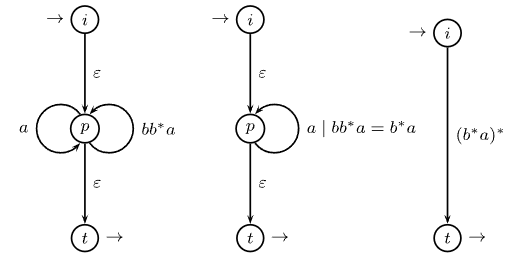
\includegraphics[width=0.6\linewidth]{images/brzozowski.png}
    \end{figure}
\end{example}